
En este capítulo definiremos los conceptos que se ven involucrados en el desarrollo de la aplicación. De esta manera podremos tener el contexto del entorno en el que nos encontramos y así comprender la importancia del uso de la tecnología actual para mejorar la comunicación entre sectores dentro de las escuelas del Instituto Politécnico Nacional.


\section{Definición de conceptos}
	\subsection{Comunicación}
	Desde tiempo atrás la comunicación ha jugado un papel de suma importancia en la vida cotidiana del ser humano, el hombre siempre se ha visto en la necesidad de comunicarse con sus semejantes con la finalidad de expresar su sentir y de esperar una respuesta, u opinión. Según Martínez y Nosnik mencionan que la comunicación es un proceso por medio del cual una persona se pone en contacto con otra a través de un mensaje, y espera que está última de una respuesta. \cite{01} Es un proceso tan simple pero a la vez primordial para la vida humana, que involucra elementos conocidos como lo son: emisor, mensaje, canal, receptor y la retroalimentación el cual se lleva a cabo entre dos o más personas.\\

%	Puedes verlo en \cite{INFLUENCIA}
	\subsection{TIC}
	Las TIC (Tecnología de la información y la comunicación) han estado presentes en la vida del ser humano desde que éste tiene la habilidad de utilizar sus recursos para comunicarse. Éstas tecnologías han ido adaptándose conforme las necesidades del ser humano, ya sea para mejorar la forma en la que nos comunicamos, hacerla más eficiente, más rápida, etc. Incluso el constante desarrollo de nuevas tecnologías han impulsado la creación de nuevas necesidades que satisfacen partcialmente por anticipado.
	 
	Las nuevas TIC agrupan los elementos y las técnicas utilizadas en el tratamiento y la transmisión de la información, principalmente de informática, internet y telecomunicaciones. El uso de las tecnologías de información y comunicación entre los habitantes de una población, ayuda a disminuir en un momento determinado la brecha digital existente en dicha localidad, ya que aumentaría el conglomerado de usuarios que utilizan las TIC como medio tecnológico para el desarrollo de sus actividades y por eso se reduce el conjunto de personas que no las utilizan. Las TIC s juegan un papel fundamental en el desarrollo del país, en razón a que son el medio masivo del futuro que logrará cerrar la brechas entre comunidades, educación, información, etc. Además de ser uno de los sectores más fuertes en el crecimiento económico de los países desarrollados, algo que deberiamos emular en los paíases en desarrollo. \cite{02}
	
	\subsection{Estilo de vida}
	Los estilos de vida se encuentran enmarcados en la interacción de las personas con la familia, trabajo, escuelas etc. En la sociedad actual según Lash y Urry, existen otras instituciones que determinan esos estilos de vida. \cite{03} Estas se encuentran fuertemente relacionadas en base a producción-consumo y tienen cabida en los medios masivos que rigen la sociedad actual. La interacción constante de las personas con estos discursos en redes masivas, provoca nichos de mercado, por lo tanto un grupo de personas que se identifican con ciertas normas de la sociedad donde se encuentran, definiendo así su estilo de vida en particular. En este punto tenemos que, en circunstancias actuales donde las personas interactúan a cada momento gracias a la tecnología, en especial a los Smartphone; esto repercute de manera directa en su estilo de vida y como se identifica con ciertos grupos de la sociedad. 
	
	Hay un término que debemos tener en cuenta y es el de la \textbf{innovación}. La innovación  es el proceso de influencia social que tiene por fuente una minoría o individuo que intenta introducir o crear nuevas ideas, nuevas modos de pensamiento o comportamiento o bien modificar ideas recibidas, actitudes y tradiciones. \cite{04}
	 
	\subsection{Smartphone (Teléfono Inteligente)}
	Si hablamos de las nuevas TIC como medio de avance en el cierre de la brecha de comunicación entre sectores, es importante,  por el objetivo de este trabajo, definidir la tecnología principal que utilizamos, los teléfonos inteligentes.
	
	Los teléfonos inteligentes se caracterizan por combinar las funciones propias de un teléfono móvil y las de una agenda electrónica. Por lo tanto un Smartphone (teléfono inteligente) debe contar con un sistema operativo el cual le permita lo siguiente:
	organizar la información personal, la instalación de aplicaciones, el intercambio de información con otros equipos, acceso a Internet a través de Wi-fi, entre muchas otras cosas. \cite{05}
	
	Los teléfonos inteligents hoy en día, son esenciales para la realización de nuestras actividades. En ellos guardamos nuestra información bancaria, los recordatorios, notas de voz, videos, imágenes, etc. Por esta razón es que esta tecnología es parte del estilo de vida del estudiante actual.

	\subsection{Aplicaciones Móviles}
	
	El uso de las aplicaciones móviles cada día toma más fuerza. Las ventajas que ofrecen los equipos inteligentes, como los smartphones o las tabletas electrónicas, han resultado de suma relevancia para diferentes ámbitos, siendo un hecho que el uso de la tecnología ha transformado de manera significativa el estilo de vida de las personas. 
	Así mismo mejorar las necesidades comunicativas que se tienen en el aspecto académico, de modo que las tecnologías de la información sirven para ayudar a la comunicación en el panorama educativo a través de la creación y el uso de herramientas tecnológicas que han permitido brindar un mejor nivel académico, poniendo al alcance diversas opciones de comunicación educativa. \cite{06}\\
	
	"Hoy en día, se puede leer el periódico, ver la cartelera del cine, ver las cuenta de banco, editar fotos, navegar en las redes sociales. No importa el lugar donde se encuentren las personas, mientras tengan un smartphone o una tablet, siempre la información estará al alcance.\\
	El desarrollo de estas aplicaciones ha surgido principalmente por la necesidad de las personas de encontrar soluciones a problemas comunes" \cite{07}

	\subsection{La comunicación en conjunto con los dispositivos móviles}
	La llegada de los teléfonos inteligentes, llámese Smartphone y tablets, ha generado el boom de los dispositivos móviles, apareciendo como el principal factor del crecimiento de la conexión de banda ancha móvil. Además de la necesidad constante de los usuarios móviles de ingresar a Internet y estar informado ha generado un crecimiento alto del consumo de Internet a través de los dispositivos móviles. \cite{09}
	\subsection{Comportamiento de los usuarios de Smartphones}
	Un estudio publicado por Google, realizado a los usuarios de Smartphones, reveló que el 81\% de los usuarios de teléfonos inteligentes navegan por Internet,  como se muestra en la figura \ref{fig:grafica1usodeinternet} de los cuales el 77\% realizan búsquedas de información, el 68\% ingresan para usar sus aplicaciones y el 48\% para visualizar vídeos en su móvil, como se muestra en la figura. \ref{fig:grafica2usodeinternet}\\ \\
	\begin{figure}[ht]
		\centering
		\caption{Usuarios Android}
		\label{fig:grafica1usodeinternet}
		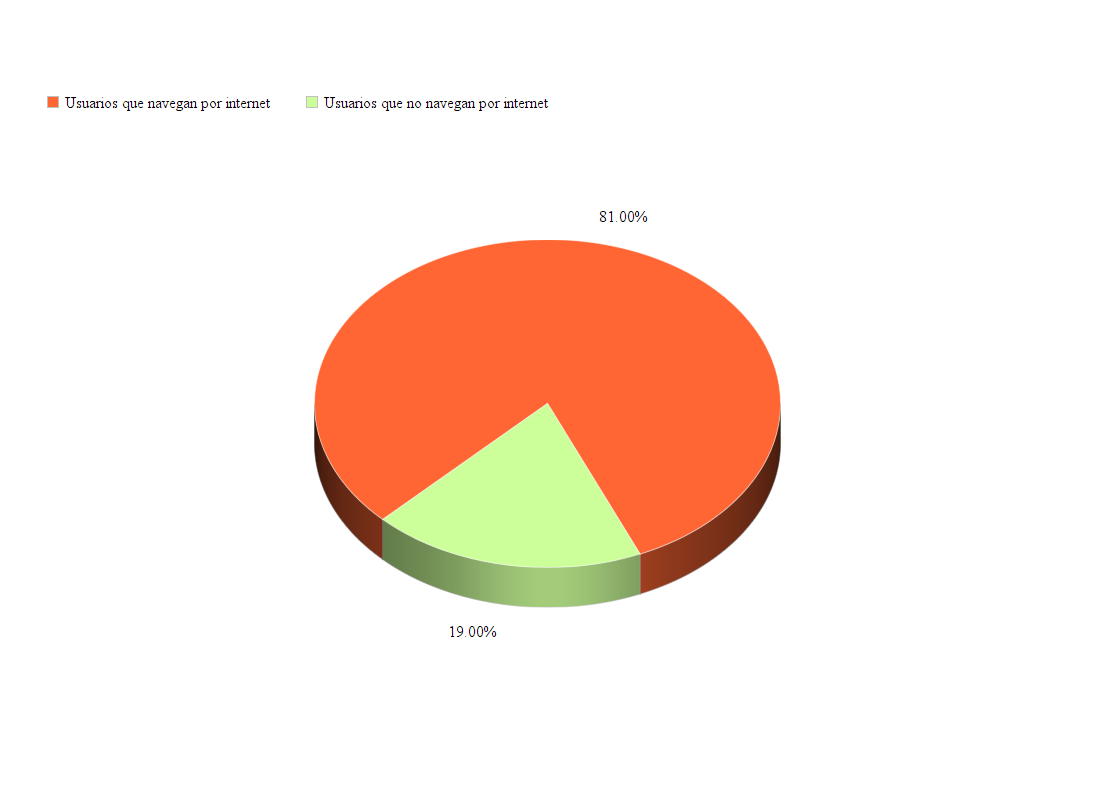
\includegraphics[width=.5\textwidth]{MarcoTeorico/usuariosusaninternet}
	\end{figure}
	\begin{figure}[ht]
		\centering
		\caption{Usuarios iOS}
		\label{fig:grafica2usodeinternet}
		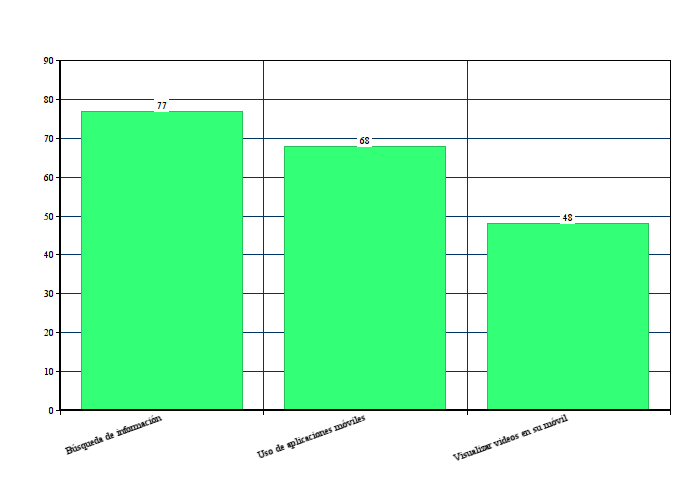
\includegraphics[width=.5\textwidth]{MarcoTeorico/usodeinterte}
	\end{figure}
	Además señalan que los consumidores utilizan sus dispositivos móviles como una extensión de sus computadoras de escritorio para realizar multi-tareas y consumir otros medios de comunicación. La investigación, también, arroja otros datos importantes como que el 72\% de los usuarios de teléfonos inteligentes usan su dispositivo mientras consumen otros medios de comunicación y el 93\% entran a Internet desde sus móviles mientras están en casa, como se muestra en la figura  \ref{fig:grafica3usodeinternet}. \cite{09} \\
	\begin{figure}[ht]
		\centering
		\caption{Gráfica de uso de internet}
		\label{fig:grafica3usodeinternet}
		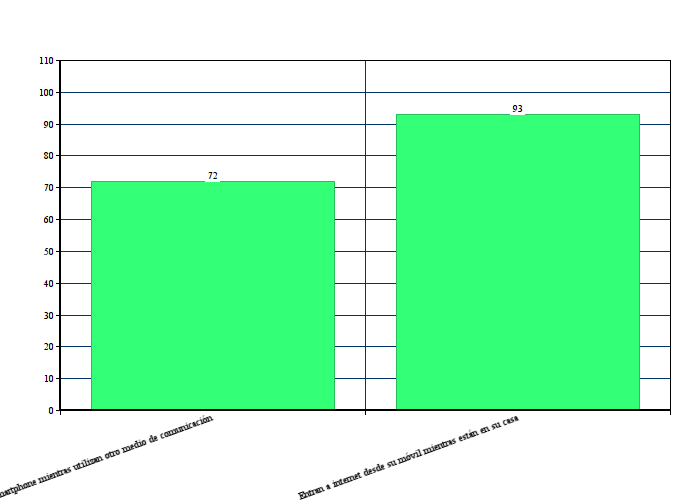
\includegraphics[width=.5\textwidth]{MarcoTeorico/usoencasa}
	\end{figure}
	
	\section{Entorno de Desarrollo}
	
		Para el presente trabajo, elegimos utilizar como plataforma de desarrollo el entorno de iOS. Siendo éste el que consideramos como la mejor opción como describimos en las siguientes secciones:
		
	\subsection{Ventajas de usar iOS}

	Curva de aprendizaje.
	Debido al tiempo que elegimos para el trabajo terminal y la definición de su cronograma, se presenta como dificultad el aprender nuevos entornos de programación, siendo ambos integrantes del trabajo afines al lenguaje de programación Swift y usuarios de la integración entre dispositivos de la marca Apple.
	
	Fragmentación de mercado.
	Al segundo trimestre del 2017 y según las aplicaciones de descarga de los sistemas operativos más usados actualmente. Google Play por parte de Android declara que el 12.3\% de sus usuarios tiene la última versión de este SO que lleva por nombre Nougat. El 32.3\% llevan la versión anterior llamada Marshmallow y el 55.4\% restante a versiones anteriores a estas (Ver figura \ref{fig:graficaandroid}). \cite{10} Por parte del SO de Apple, el 87\% de sus usuarios activos cuenta con la versión más reciente iOS 10, el 10\% la versión anterior iOS 9 y el 3\% restante una versión anterior (Ver figura \ref{fig:graficaiost}). 
		\begin{figure}[ht]
		\centering
		\caption{Gráfica de uso de internet}
		\label{fig:graficaiost}
		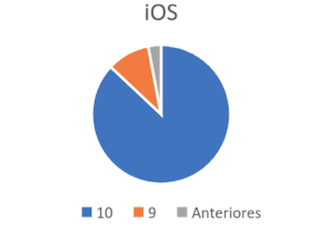
\includegraphics[width=.5\textwidth]{MarcoTeorico/iosgrafica}
	\end{figure}
\begin{figure}[ht]
	\centering
	\caption{Gráfica de uso de internet}
	\label{fig:graficaandroid}
	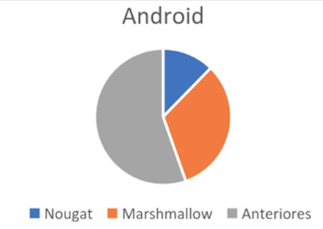
\includegraphics[width=.5\textwidth]{MarcoTeorico/androidgrafica}
\end{figure}


	Con la información anterior, consideramos que es importante desarrollar para dispositivos a los cuales el usuario final pueda estar siempre actualizado, esto permite la mejora continua de la aplicación y un mayor alcance en ámbito de usuarios que puedan tener acceso a la escalabilidad del proyecto en un futuro.
	\subsection{Sistema operativo iOS}
	iOS (anteriormente denominado iPhone OS) es un sistema operativo móvil de Apple desarrollado originalmente para el iPhone, siendo después usado en el iPod Touch e iPad. Es un derivado de Mac OS X, que a su vez está basado en Darwin BSD. El iOS tiene 4 capas de abstracción: la capa del núcleo del sistema operativo, la capa de "Servicios Principales", la capa de "Medios de comunicación" y la capa de "Cocoa Touch". Todo el sistema se encuentra en la partición "/root" del dispositivo, ocupa poco menos de 500 megabytes. También llamado D-IOS por sus fans. \cite{11}\\ \\
	Historia del iOS\\
	Apple reveló la existencia de iPhone OS en la Macworld Conference y Expo del 9 de enero de 2007, aunque el sistema no tuvo un nombre oficial hasta que salió la primera versión beta del iPhone SDK un año más tarde, el 6 de marzo de 2008. Antes de esto se consideraba simplemente que el iPhone corría OS X. A partir de entonces se llamaría iPhone OS. El lanzamiento del iPhone OS tuvo lugar el 29 de junio de 2007. El interés en el SDK aumentaría en meses siguientes debido al explosivo crecimiento de la plataforma iPhone, que se vio incrementado en septiembre de 2007 del iPod Touch, un dispositivo con las capacidades multimedia del iPhone pero sin la capacidad de hacer llamadas telefónicas. \cite{12}\\
	
	El 27 de enero de 2010 Steve Jobs, CEO de Apple, anunció el iPad, un dispositivo muy similar al iPod Touch pero con un enfoque más orientado hacia la industria de contenidos. Este dispositivo, apoyado en una pantalla táctil algo mayor, compartiría sistema operativo con sus dos exitosos hermanos, y vendría acompañado de una aplicación oficial para la compra y lectura de libros electrónicos, iBooks. A fecha de abril de 2010 se estima por encima de 185.000 las aplicaciones disponibles para iPhone OS a través de la App Store. El 7 de junio de 2010, durante la presentación del iPhone 4, Steve Jobs anunció que iPhone OS pasaría a ser llamado oficialmente como iOS. \cite{12}
	\subsection{Características}
	La interfaz de usuario de iOS se basa en con el concepto de manipulación mediante gestos multitáctil. Los elementos de la interfaz se componen por deslizadores, interruptores y botones. La respuesta es inmediata y se provee de una interfaz fluida. La interacción con el sistema operativo se realiza mediante gestos como deslizar, tocar y pellizcar. Acelerómetros y Giroscopios internos son utilizados por algunas aplicaciones para responder a movimientos y gestos, como sacudir el aparato (en campos de texto es usado para deshacer y rehacer) o rotarlo (se suele usar para cambiar de posición vertical a modo paisaje). \cite{13}\\
	
	La pantalla principal (llamada «SpringBoard») es donde se ubican los iconos de las aplicaciones y el Dock en la parte inferior de la pantalla donde se pueden anclar aplicaciones de uso frecuente, aparece al desbloquear el dispositivo o presionar el botón de inicio. La pantalla tiene una barra de estado en la partes, historia pasada y futuro inmediato superior para mostrar datos, tales como la hora, el nivel de batería, y la intensidad de la señal. Todas las «utilidades», como Notas de Voz, Reloj, Brújula y Calculadora están en una carpeta llamada «Utilidades» desde la versión 4.0. Varias de las aplicaciones incluidas están diseñadas para trabajar juntas, permitiendo compartir datos de una aplicación a otra. (Por ejemplo, un número de teléfono puede ser seleccionado desde un email y guardarlo como un contacto o para hacer una llamada). El iPod Touch tiene las misma apps que están presentes en el iPhone, con excepción de Teléfono, Mensajes y Brújula.\\ 
	
	La aplicación iPod está separada en dos apps diferentes: Música y videos. Los iconos en el dock se usan para mostrar las funciones principales del iPod Touch: Música, Vídeos, Safari y App Store. El iPad también tiene las mismas aplicaciones que el iPhone, excluyendo Bolsa, Tiempo, Reloj, Calculadora, Voice Memos, Teléfono, Mensajes y Nike+iPod, apps separadas para música y vídeo igualmente se usan (como en el iPod Touch), pero la aplicación de música esta denominada como iPod. Varias apps por defecto están reescritas para tomar ventaja de la pantalla más grande. El dock por defecto incluye Safari, Mail, Fotos y iPod.\\ \\
	Multitarea 
	
	Antes de iOS 4, la multitarea estaba reservada para aplicaciones por defecto del sistema. A Apple le preocupaba los problemas de batería y rendimiento si se permitiese correr varias aplicaciones de terceros al mismo tiempo. A partir de iOS 4, dispositivos de tercera generación y posteriores soportan el uso de 7 APIs para multitarea, específicamente:
	1. Audio en segundo plano 48
	2. Voz IP
	3. Localización en segundo plano
	4. Notificaciones push
	5. Notificaciones locales
	6. Completado de tareas
	7. Cambio rápido de aplicaciones
	
	Sin embargo, no consiste en una verdadera multitarea, pues las aplicaciones ajenas al SO, quedan congeladas en segundo plano no recibiendo un solo ciclo de reloj del procesador. \cite{14}
	
%	\section{Problemática y solución propuesta}
%		La comunicación dentro de la comunidad estudiantil de la Escuela Superior de Cómputo (ESCOM) es un tema de controversia. Actualmente existen problemas de comunicación de los alumnos con los profesores, así como con muchas de las áreas que tiene la institución.\\
%	
%	En la Escuela Superior de Cómputo (ESCOM) existen problemas de comunicación y de la manera en como fluye la información que va destinada hacia la comunidad estudiantil, estos problemas influyen en la vida académica de los alumnos tales como:
%	\begin{itemize}
%		\item \textbf{\textit{La dificultad de localizar las áreas o espacios de la Escuela Superior de Computo.}}\\
%		
%		Este es uno de los principales problemas a atacar, ya que las áreas de la institución causa confusión a los alumnos de nuevo ingresó o personas visitantes a la institución y es complicado saber la localización exacta de las áreas de la ESCOM así como entender la nomenclatura de los salones, incluso existen alumnos que tienen mas tiempo dentro de la institución y aún les genera confusión la nomenclatura que utiliza la institución.\\ 
%		
%		Los salones tienen dos nomenclaturas. Definida para los salones de la siguiente manera:
%		\begin{itemize}
%			\item Número de edificio
%			\item Número de piso
%			\item Número de salón
%		\end{itemize}
%		
%		Como se muestra en el ejemplo \textit{1a \textbf{2201}}.
%		
%		Donde el primer \textbf{2} de izquierda a derecha es el número de edificio de la institución, el segundo \textbf{2} es el piso del edificio y finalmente el \textbf{01} es el número del salón.\\
%		
%		\begin{itemize}
%			\item Número de salón
%			\item Letra 'N' para "Norte"  y  'S' para "Sur" de acuerdo a  la ubicación del salón
%		\end{itemize}
%		
%		Como se muestra en el ejemplo \ref{ejemplo2}{1b} \textbf{21N} \label{ejemplo2} 
%		
%		Donde el número \textbf{21} indica el número de salón y \textbf{N} que indica que el salón esta orientado hacia el Norte\\
%		
%		Otro de los problemas que existen es que los alumnos no conocen la ubicación de las areas de la ESCOM, tales como: Dirección, Subdirección Académica, Coordinación de Desarrollo Tecnológico, Recursos Materiales, Decanato.\\ 
%		
%		En la entrada principal de la Escuela Superior de Cómputo existe un mapa de localización de las áreas de la escuela el cual no contempla todas las áreas existentes.  Lo que nos genera problemas de comunicación entre la institución y las personas que están en ellas. \\ Impuntialidad ya que puede tomar unos minutos ubicar el salón o el área que se desea. En la temporada de inicio de semestre, durante la primer semana uno de los problemas es la mala difusión de los salones donde se impartirán las clases lo que implica perdida de tiempo al buscar la ubicación del salón asignado, perdida de tiempo al buscar la pancarta impresa de la asignación de los salones.\\ \\
%		
%		\item \textbf{\textit{Complicaciones al obtener material educativo.}} \\
%		
%		Si bien es cierto, el ser autodidacta es uno de los puntos mas importantes que debe tener un estudiante de la ESCOM para poder complementar su desarrollo académico, la falta de material educativo fuera de la ESCOM para los alumnos es complicada, ya que existen pocos elementos extracurriculares.\\
%		
%		Dentro de la institución se maneja una herramienta llamada Moodle, la cuál es una aplicación dirigida a la educación que ayuda a contrarrestar este tipo de necesidades, sin embargo, esta está dirigida solo a los alumnos cuyos profesores tengan acceso y hagan uso a esta herramienta. La cuál usualmente es utilizada como plataforma de entregas o evaluaciones de actividades dejando lejos el material educativo para que los alumnos puedan aclarar o practicar los temas vistos en clase. \\
%		
%		La ayuda de un elemento que auxilie a los alumnos ayudaría de manera significativa a mejorar el nivel académico de los mismos, facilitando la etapa de evaluaciones que se llevan a cabo a lo largo del semestre escolar.\\ \\
%		
%		\item \textbf{\textit{Dificultad en la  difusión de cursos y certificaciones gratuitas para los alumnos de la ESCOM y desaprovechamiento de los mismos por parte de los alumnos.}}\\
%		
%		La Escuela Superior de Cómputo oferta una gran variedad de cursos y certificaciones para sus alumnos tanto gratuitas como con algún costo, sin embargo son desaprovechadas por una gran cantidad de alumnos debido a que en ocasiones estos ni se enteran de los cursos que se ofrecen. Esto produce un gran desperdicio de oportunidades de crecimiento académico para los alumnos.\\
%		
%		Los cursos que se ofertan en la ESCOM en su mayor parte son difundidos dentro de la escuela mediante ferias, folletos o carteles entre otros, los cuales en su mayoría de veces son ignorados por la comunidad por la falta de interés hacia este tipo de "propagandas", como se mencionada en el párrafo anterior, esto desencadena una falta de aprovechamiento importante.
%		
%		Una solución propuesta es agregar otros tipos de difusiones para dirigirlas a los alumnos y estos puedan hacer de su conocimiento de todas las oportunidades que oferte la ESCOM. El poder visualizar desde tu dispositivo móvil todas aquellas certificaciones o cursos podrían llevar al alumnos a tomarlos, si estos cursos son de su interés. Teniendo la posibilidad de tener una mejor cantidad de alumnos inscritos a este tipo de actividades escolares.\\ 
%		
%		
%		
%		\item \textbf{\textit{Mala difusión de los procesos relacionados con Movilidad Estudiantil.}}\\
%		
%		Este punto esta un poco relacionado con el anterior, puesto que en la ESCOM existe la posibilidad para los alumnos de dirigirse a otra universidad en calidad de movilidad estudiantil y vivir la experiencia de estudiar ya sea fuera de la ciudad o en el extranjero. \\
%		
%		La falta de comunicación entre este proceso y los alumnos, genera controversia y confusiones con los mismos, ya que en ocasiones no saben las fechas de convocatoria ni los requisitos que se necesitan para aplicar una movilidad. Esta oportunidad tan grande que brinda tanto el IPN como la ESCOM es de suma importancia y se debe fomentar aún mas esta oportunidad para poder dar renombre de la calidad estudiantil del instituto y de los mexicanos.\\
%		
%		Es por eso que se propone que las aplicaciones móviles funcionen como medio de difusión de convocatorias y requisitos así como de los lugares en donde se puede realizar la movilidad y así darle esa gran oportunidad a los alumnos de aprender de otras culturas y de como es realizar una vida en el extranjero.\\
%		
%	\end{itemize}
%	
%	Es por eso que en este Trabajo Terminal se propone una aplicación móvil para ayudar al buen flujo de información y a la buena comunicación con la comunidad de la Escuela Superior de Computo para facilitar la vida académica de los alumnos y resolver los problemas mencionados anteriormente.\\
%	
%	La aplicación móvil propuesta anteriormente permitirá un mejor seguimiento y comunicación para la comunidad estudiantil de la Escuela Superior de Computo (ESCOM).\\
%	
%	Con base en las necesidades de la comunidad estudiantil de la Escuela Superior de Cómputo se pretende crear una aplicación móvil que contemple principalmente las siguientes características:
%	\begin{itemize}
%		\item Consulta de horario.
%		\item Consulta de los medios de contacto del personal docente.
%		\item Consulta del listado de asignaturas impartidas durante el semestre.
%		\item Noticias Académicas.
%		\item  Consulta de material educativo.
%	\end{itemize}
